\documentclass[journal]{IEEEtran}

% Packages
\usepackage{cite}
\usepackage{graphicx}
\usepackage{subfigure}
\usepackage{float}
\usepackage{url}
\usepackage{color}
\usepackage{amsmath}


\begin{document}

% paper title
% can use linebreaks \\ within to get better formatting as desired
\title{Probabilistic~Robotics~Lab~4 \\ Extended~Kalman~Filter}
%

\author{Rodrigo~Caye~Daudt}





% make the title area
\maketitle



%%%%%%%%%%%%%%%%%%%%%%%%%%%%%%%%%%%%%%%%%%%%%%%%%%%%%%%%%%%%%%%%%%%%%%%%%%%%%%%
\section{Introduction}

\IEEEPARstart{T}{his} report describes the work done for lab 4 on the Probabilistic Robotics module, for which an Extended Kalman Filter (EKF) was developed in Python to work with ROS simulations. Section \ref{ekf} briefly describes EKFs and gives some information about our implementation. Section \ref{results} shows and analyses the results obtained by using the developed filter. Section \ref{conclusion} closes this work with the main observations and conclusions.

%%%%%%%%%%%%%%%%%%%%%%%%%%%%%%%%%%%%%%%%%%%%%%%%%%%%%%%%%%%%%%%%%%%%%%%%%%%%%%%
\section{Extended Kalman Filter}\label{ekf}

The Extended Kalman Filter is a localization filter used to merge the different types of data available to a robot's controller. The EKF uses a Gaussian vector to describe the robot's state along with the estimated uncertainty at any point in time. EKFs are therefore unimodal filters, unlike the Bayes filter or the particle filter, and need a decent initial estimation of the robot's state.

The first step in applying an EKF is to model the behaviour and measurement of the robot. Our model for the behaviour of the turtlebot is defined in Equations \ref{f} to \ref{H2}. These equations model the prediction of the position of the turtlebot given a previous position, a control signal and an odometry measurement. The equations also model the measurements performed by the turtlebot at a given state. More information about the modelling can be found in the pre-lab report.

\begin{align}\label{f}
\hat{x_k} = 
\begin{bmatrix}
\hat{x}_{r_{k-1}} + \Delta x \cdot cos \theta_{k-1} - \Delta y \cdot sin \theta_{k-1} \\
\hat{y}_{r_{k-1}} + \Delta x \cdot sin \theta_{k-1} + \Delta y \cdot cos \theta_{k-1} \\
\theta_{k-1} + \Delta \theta
\end{bmatrix}
\end{align}



\begin{align}\label{A}
A_k = 
\begin{bmatrix}
1 & 0 & -\Delta x\cdot sin \theta_{k-1} - \Delta y \cdot cos \theta_{k-1} \\
0 & 1 & \Delta x\cdot cos \theta_{k-1} - \Delta y \cdot sin \theta_{k-1} \\
0 & 0 & 1 \\
\end{bmatrix}
\end{align}

We define $\rho_r '$ as 

\begin{align}\label{rho}
\rho_r ' = \rho_w - x_r cos\phi_w - y_r sin \phi_w
\end{align}

If $\rho_r ' >= 0$:

\begin{align}\label{h1}
h(x_k,v_k) = 
\begin{bmatrix}
\rho_w - x_r cos\phi_w - y_r sin \phi_w + v_\rho \\
\phi_w - \theta
\end{bmatrix}
\end{align}

\begin{align}\label{H1}
H_k = 
\begin{bmatrix}
-cos\phi_w & -sin \phi_w & 0 \\
0 & 0 & -1
\end{bmatrix}
\end{align}

If $\rho_r ' < 0$:

\begin{align}\label{h2}
h(x_k,v_k) = 
\begin{bmatrix}
-\rho_w + x_r cos\phi_w + y_r sin \phi_w + v_\rho \\
\phi_w - \theta + \Pi
\end{bmatrix}
\end{align}

\begin{align}\label{H2}
H_k = 
\begin{bmatrix}
cos\phi_w & sin \phi_w & 0 \\
0 & 0 & -1
\end{bmatrix}
\end{align}

Once we have data from the internal sensors, we can apply the prediction step of the EKF. This step is defined by the block of equations starting at Eq. \ref{eq:pre}. This step predicts a new position as best as possible with the available information. In this step the covariance matrix is also modified to incorporate the new uncertainty from the motion estimation.

\begin{align}\label{eq:pre}
& x_{k|k-1} = f(x_{k-1},u_k , w_k)\\
& P_{k|k-1} = A_k P_{k-1} A_k^T + W_k Q_k W_k^T
\end{align}


Once data from the external sensors is available we can continue with the EKF operations. Since we are comparing our measurements to a line based map, we need to compare the measured lines to the map lines and find the best fit. For this, we use the Mahalanobis distance to calculate in a fair way the distance between the two lines. Mahalanobis distance is used to weigh differently the distance $\rho$ and the angle $\phi$ of the lines to obtain a more fair comparison. If no line is a good fit for the measured line, the measurement is discarded. This step is accomplished by the operations described in the block of equations starting at Eq. \ref{eq:ass}.

One extra step was taken here to avoid matching measurements to ghost lines. Since the polar representation of the lines contains no information about the start and the end of the lines, we separately calculated the size of the measured and map lines and compared these values to increase the precision of the data association step. If the measured line was bigger than the best match in the map lines, the measurement would be discarded since that was not possible. An error margin of 10\% was used to cope with the measurement errors and the imprecision of the split and merge algorithm.

\begin{align}\label{eq:ass}
& v_{ij} = z_i - h(x_{k|k-1})\\
& S_{ij} = H_j P_{k|k-1} H_j^T + R_i\\
& D_{ij}^2 = v_{ij}^T S_{ij}^{-1} v_{ij}\\
& Take~the~smallest~D_{ij}^2~if~D_{ij}^2<\chi_{\rho,\phi}^2
\end{align}

Finally, once the data association has been performed and the best fit for each measured line has been found, we can perform the update step. This step merges the predicted state with all the measurements, using all the available data to calculate the best prediction with the given data. Once again, the state of the robot and the covariance matrix are modified, resulting in a more precise state estimation and to express the uncertainty of the current state estimation.This step is accomplished by the operations described in the block of equations starting at Eq. \ref{eq:up}.

\begin{align}\label{eq:up}
& v_k = z_k - h(x_{k|k-1})\\
& S_k = H_k P_{k|k-1} H_k^T + R_k\\
& K_k = P_{k|k-1} H_k^T S_k^{-1}\\
& x_k = x_{k|k-1} + K_k v_k\\
& P_k = (I-K_k H_k)P_{k|k-1}(I-K_k H_k)^T+K_k R_k K_k^T
\end{align}


These steps were performed in a loop as fast as the computer and the sensor data allowed in order to obtain a very good state estimation at all times.




%%%%%%%%%%%%%%%%%%%%%%%%%%%%%%%%%%%%%%%%%%%%%%%%%%%%%%%%%%%%%%%%%%%%%%%%%%%%%%%
\section{Tests and Results}\label{results}

\begin{figure*}[ht]
	\centering

	\subfigure[$t_1$]{\label{ekf1}
		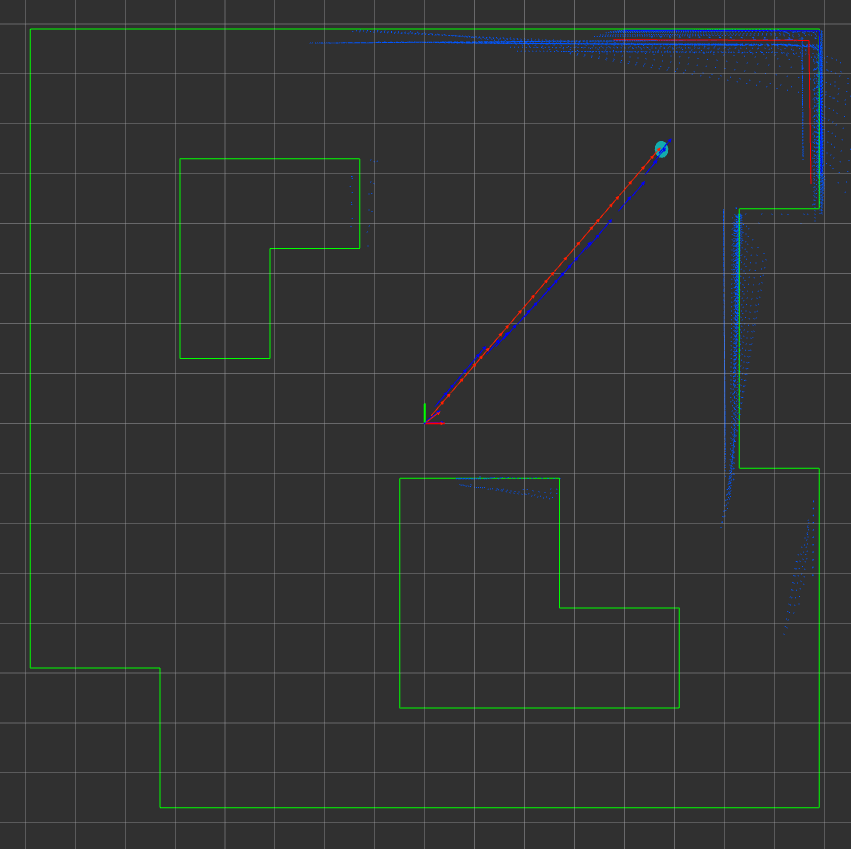
\includegraphics[width=0.45\linewidth]{figures/ekf1.png}}~
	\subfigure[$t_2$]{\label{ekf2}
		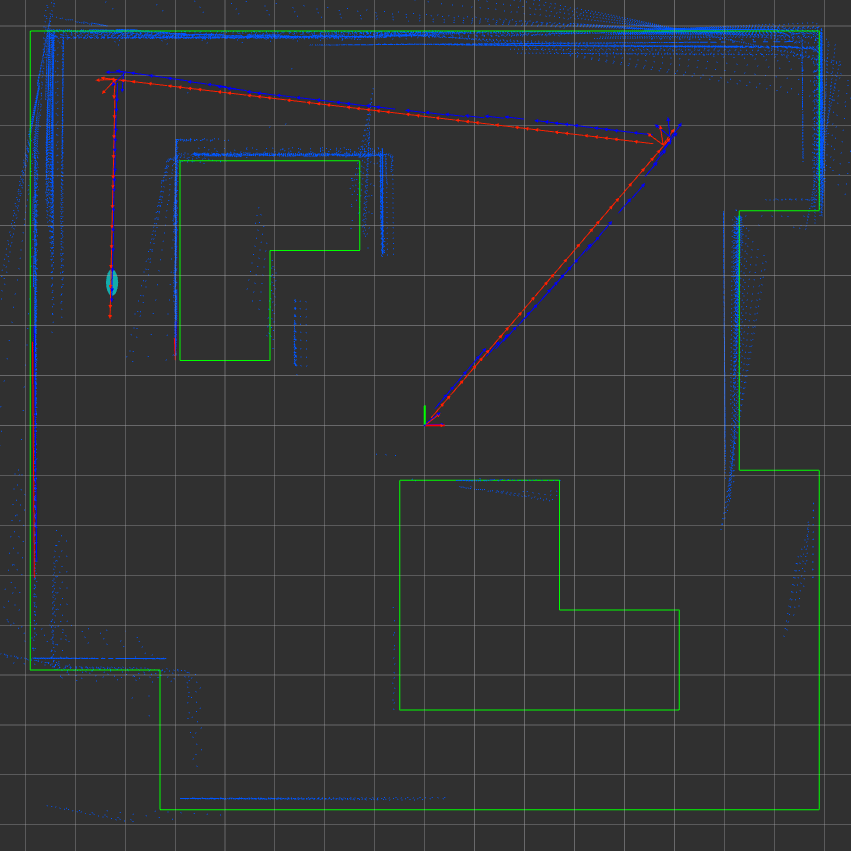
\includegraphics[width=0.45\linewidth]{figures/ekf2.png}}\\

	\subfigure[$t_3$]{\label{ekf3}
		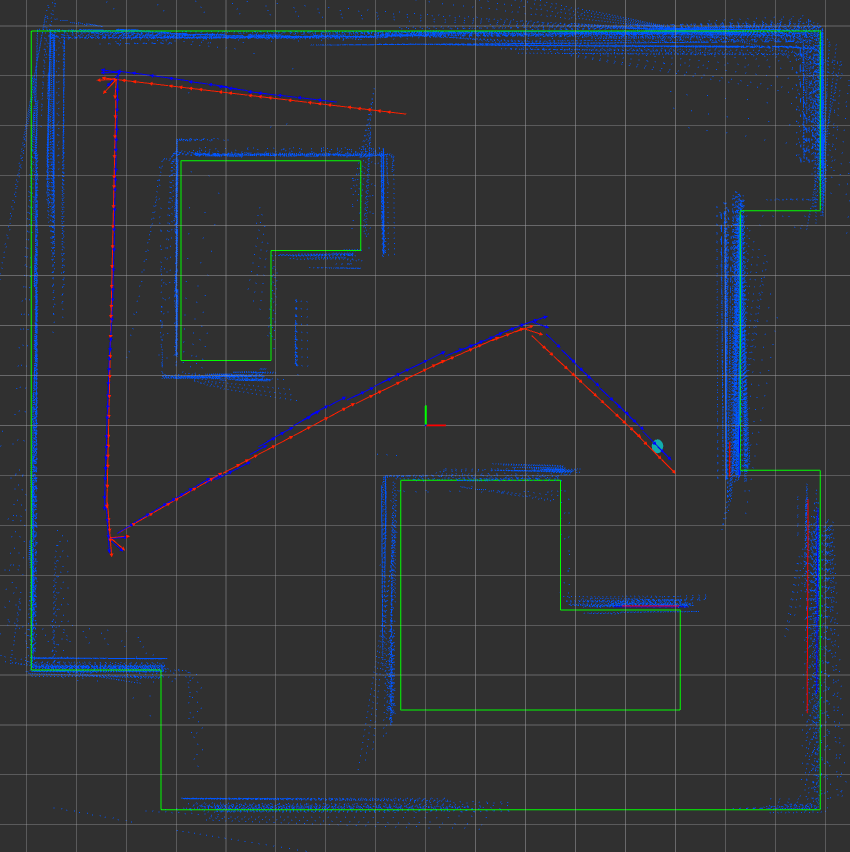
\includegraphics[width=0.45\linewidth]{figures/ekf3.png}}~
	\subfigure[$t_4$]{\label{ekf4}
		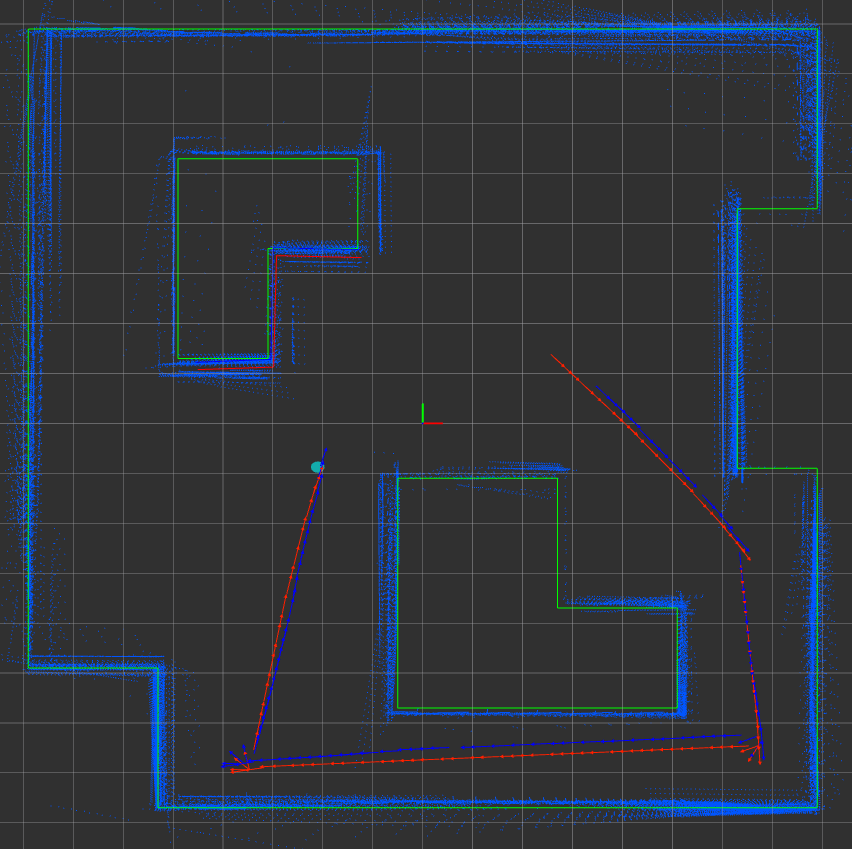
\includegraphics[width=0.45\linewidth]{figures/ekf4.png}}\\

	\caption{Simulation of the EKF at four different simulation times}
	\label{fig:ekf}
\end{figure*}

The implemented EKF was tested using pre recorded data from a turtlebot simulation in a known environment. This simulation is shown in Fig. \ref{fig:ekf}, where four different stages of the simulation are displayed in \ref{ekf1} to \ref{ekf4}. In the images, we can see the following things:

\begin{itemize}
	\item The map lines in green
	\item The trajectory given only by the odometry in red arrows
	\item The trajectory corrected by the EKF in dark blue arrows 
	\item The uncertainty at the current state as a light blue ellipse
	\item The measurements made by the turtlebot relative to the EKF predicted state as blue dots
	\item The lines obtained from the split and merge function using the external sensor data as red lines
\end{itemize}

We can see that the EKF is a very good way to merge all the available data into one coherent state prediction, as is demonstrated by how the blue dots are close to the map lines. We can see that the uncertainty at every step is very small, which helps with the robot's navigation.

During the simulation we could see that the uncertainty regarding the robot's state grew when there was not much data from the external sensors, but the state prediction would recover quickly once a wall was observed once again. We could also observe that the data would be very poor when the robot turned, seen that at those moments the observed data would differ dramatically from the map lines. But once again, the state would recover very well once the robot had walls to observe and match to the known map.







%%%%%%%%%%%%%%%%%%%%%%%%%%%%%%%%%%%%%%%%%%%%%%%%%%%%%%%%%%%%%%%%%%%%%%%%%%%%%%%
\section{Conclusion}\label{conclusion}

In this work we developed an EKF to help us predict the current state (position and direction) of the turtlebot. We observed that although being mathematically complex, the operations performed in an EKF are not too complex and result in a way to associate different types of data with relatively low computational effort compared to other options such as the Bayes filter or the particle filter. It is computationally efficient since it compresses all the uncertainty into the parameters of the Gaussian vectors instead of fully describing an arbitrary probability density function.

We also observed no problems regarding the stability of the EKF, since it performed well in all runs of the program. That is not the case for a particle filter, for example, which being a stochastic filter may have weird behaviours if not enough particles are used. This is mainly a consequence of the EKF being a deterministic filter, i.e. it uses no random sampling of any kind.



%\bibliographystyle{IEEEtran}
%\bibliography{Template_Daudt}


\end{document}


